\chapter{仿冒开发者行为特征实证分析}
\label{chp:discoveries_behavior}

本章针对仿冒应用开发者的行为特征进行实证研究,了解该类行为有助于了解应用市场现有监管机制是否存在缺陷,从而可针对性地提出改善措施。
研究内容主要为分析仿冒应用与开发者的对应关系、仿冒应用证书活跃期、仿冒应用上架速度等与开发者行为相关的方面。
具体分析从三部分展开,结合应用证书视角与结合时间维度视角进行探索,对应以下三个研究问题:

\textbf{ RQ4:仿冒应用与开发者的对应关系如何?}

\textbf{ RQ5:仿冒应用证书可以活跃多长时间?}

\textbf{ RQ6:仿冒应用的上架行为是否有特征?}

\section{研究方法}
\label{sec:behavior_method}

本节介绍本章研究中整理研究数据的方法,以讨论研究的结构有效性。
对RQ4,根据~\secref{sec:signature}的介绍,可利用样本的应用证书构建其与应用开发者的对应关系,RQ5亦涉及应用证书相关信息使用,因此需要阐明应用证书数据的获取方式;
同时,RQ5有对应用证书活跃时间的需求,本章研究引入了一个应用证书活跃时间的近似计算方法;
对RQ6,为研究仿冒引用的上架特征,本研究整理复原了各款正版应用各版本上架的时间线,本节将介绍时间线的整理方法。
本章研究对象为与上一章相同、由69,414个正版样本与52,638个仿冒样本组成的应用集。

由~\secref{sec:signature},可知每个APK文件内都有包含应用开发者信息的\textit{CERT.RSA}文件。
每个仿冒样本,作者将其解压,取出\textit{/META-INF}文件夹中的应用证书文件,再利用Keytool~\cite{keytool}工具获取证书信息(如\textit{应用证书SHA1码}与\textit{应用开发者名})。
Keytool工具为Java自带工具,被广泛地用于管理密钥和证书,因此可相信使用Keytool获取的应用证书信息无误。

在获取应用证书活跃度方面,由于Janus类似一个爬取各大市场应用的平台,并不能感知某样本的下架时间或某样本是否已下架,因此只能对仿冒应用证书的活跃时间作近似计算。
计算的具体方法为将所有仿冒样本遍历一次,取出样本的应用证书SHA1码,凭借该样本的搜集时间更新该应用证书的最早出现时间(或最晚出现时间),取各证书最早出现时间与最晚出现时间为证书的活跃期,活跃期长度则为该证书的活跃时长。

为了解仿冒应用的上架速度,研究需要获取各款目标应用每个版本的更新时间和与该版本对应的仿冒样本的上架时间。
各个目标应用多年来发布版本众多,已无法从大部分应用官网中寻回完整更新日志,因此本研究借助样本集中的正版样本搜集时间整理复原各版原版应用的上架时间线。
本文对所有收集到的正版样本按目标应用进行分类,再按照版本号对同一目标应用下所有样本排序。
由于同一应用可在多个市场上架,同一版应用在不同市场可能存在细小差别(如在华为市场上架的应用需要接入华为钱包作为支付途径),导致同一版本的APK安装包具有不同SHA1码。
因此,此处以应用版本而非应用SHA1码为粒度分割样本,以消除上述情况影响。
另外,基于各市场审核流程、其他商业因素考虑,可能存在应用同一版本在不同市场有不同上架时间的情况。
针对该情况,如某版原版样本存在多个上架时间,本研究只取最小值,该值表示仿冒应用开发者可接触该版原版应用的最早时间。
之后,将每款应用中每个版本上架时间串联,即可大致重现每款应用的更新时间线。

从仿冒样本角度考虑,仿冒样本大多不是重打包应用,无法与原版应用的版本号直接对应。
为求出仿冒样本的仿冒延迟(即原版应用上架时间与仿冒样本上架的时间差),本文提取出每个仿冒样本的上架时间,以不晚于这个仿冒样本发布的原版应用作为其对应的仿冒对象,取两者上架时间差作为仿冒延迟。

\section{实证研究流程与结果解析}

本节分为四个部分,前三个部分分别对应本章三个研究问题的研究流程,最后一部分对本章研究进行有效性分析。

\subsection{应用证书与仿冒应用对应关系}

\noindent{\bf RQ4:仿冒应用与开发者的对应关系如何?}

由于每个仿冒样本均有对应的应用证书,本研究构造了仿冒样本与应用证书的二分图,其中两类节点分别为仿冒样本和应用证书,若两节点之间存在边,则表示该样本由该证书签署。
在仿冒应用持有的所有应用证书中,多数证书(76\%)仅仅关联了一个或两个仿冒样本,与最多仿冒应用的证书签署了1,374个仿冒样本。
\autoref{table:certificate_number_statistic}统计了应用证书和他们对应的仿冒样本数量。
表格第一栏为仿冒样本的数量区间,第二栏为关联的仿冒样本数量该落于区间的应用证书数,如第一列数据指有8,252个应用证书签署的样本数为1到5个。
大部分应用证书都只关联了1到5个应用样本,但也有少量应用证书与大量仿冒样本有关联关系。

\begin{table}[htbp]
    \renewcommand{\arraystretch}{1}
    \footnotesize
    \centering
    \caption{应用证书/仿冒应用数量对应表}
    \vspace{1mm}
    \begin{tabular}{l c c c c c c c}
        \toprule
        {\bf 关联仿冒样本数量} & {\bf 1-5} & {\bf 6-10} & {\bf 11-50} & {\bf 51-100} & {\bf 大于100} \\
        \midrule
        {\bf 应用证书数量}     & 8252      & 525        & 531         & 71           & 80            \\
        \bottomrule
    \end{tabular}
    \label{table:certificate_number_statistic}
\end{table}

鉴于应用证书与应用开发者存在多对一关系(\secref{sec:signature}Android App签名机制),作者认为每个应用证书只签署少量样本是仿冒应用开发者规避应用市场监管机制的策略。
如果仿冒应用开发者只使用一个应用证书上传多个仿冒应用,万一其中一个应用被投诉下架,使用同一证书签署的其他的应用很可能会受到牵连。
但一个仿冒应用开发者可持有多个应用证书,即仿冒应用开发者可利用多个身份在应用市场中上传应用,继而令应用市场就难以找到仿冒应用之间的关联。
即使其中一个证书签署的仿冒应用被举报下架,由其他证书签署的余下应用也得以被保全。

另一方面,有部分仿冒应用应用证书与多个仿冒样本关联。
其中,SHA1码为``\emph{61ed377e85d386a8dfee6b864bd85b0bfaa5af81}''的应用证书是所有证书中关联仿冒样本最多的,有1,374个样本由该应用证书签署,样本涵盖了本研究数据集47个目标应用中的37个(79\%)。
根据Keytool从该证书抽取出的开发者信息,其开发者名为``Android''。
Android官方文档~\cite{UICCcert}显示,该证书为Android Studio自带的Android调试证书。
此结果表明国内大部分应用市场在审核阶段并未对该类证书进行有效拦截,开发者可凭借该类证书将仿冒应用上传至市场中,增加用户风险。

进一步,作者抽取所有证书的开发者名称进行匹配,得到~\autoref{table:certificate_developer_name}。
与下文~\autoref{table:certificate_number_statistic}相似,表格第一栏为某开发者名对应应用证书的数量区间,第二栏为对应应用证书数量该落于区间的开发者名称数,如第一列数据指有5,355个开发者名称仅与1个应用证书对应。

\begin{table}[htbp]
    \renewcommand{\arraystretch}{1}
    \footnotesize
    \centering
    \caption{应用证书数量/开发者名称数量对应表}
    \vspace{1mm}
    \begin{tabular}{l c c c c c c c}
        \toprule
        {\bf 对应应用证书数量} & {\bf 1} & {\bf 2-5} & {\bf 6-10} & {\bf 11-50} & {\bf 大于50} \\
        \midrule
        {\bf 开发者名称数量}   & 5355    & 419       & 38         & 23          & 9            \\
        \bottomrule
    \end{tabular}
    \label{table:certificate_developer_name}
\end{table}

对应证书最多的前10个开发者名称与其对应证书数量依次为:\emph{cn}(873),\emph{Android Debug}(441),(空字符串)(279),\emph{Unknown}(207),\emph{mobcent}(195),\emph{addone}(125),\emph{Java}(102),\emph{Android}(63),\emph{1}(56),\emph{a}(43),其中\emph{Android Debug}、\emph{Android}为Android调试证书的开发者名,\emph{Java}很可能为利用Keytool生成证书的默认开发者名,空字符串、\emph{cn}与\emph{Unknown}为其他工具生成证书的默认开发者名(CN对应生成证书时需输入的开发者昵称,Common Name),\emph{1}、\emph{a}也不是有意义的开发者名称。
因此,除\emph{addone}与\emph{mobcent}两个开发者名称有具体含义外,余下8个开发者名称无明显意义,即其对应的应用证书很可能为调试证书。

\begin{table}[htbp]
    \renewcommand{\arraystretch}{1}
    \footnotesize
    \centering
    \caption{开发者名称/仿冒样本数量对应表(关联数前十位)}
    \vspace{1mm}
    \begin{tabular}{l c}
        \toprule
        {\bf 开发者名称}                        & {\bf 对应仿冒样本数量} \\
        \midrule
        cn                                      & 1,888                  \\
        \rowcolor{gray!15}Android               & 1,661                  \\
        Android Debug                           & 1,285                  \\
        \rowcolor{gray!15}(空字符串)          & 1,278                  \\
        zh                                      & 1,176                  \\
        \rowcolor{gray!15}http://soft.sj.91.com & 1,033                  \\
        yk                                      & 982                    \\
        \rowcolor{gray!15}Gavin Van             & 698                    \\
        Unknown                                 & 653                    \\
        \rowcolor{gray!15}android               & 560                    \\
        \bottomrule
    \end{tabular}
    \label{table:developer_name_sample_cnt}
\end{table}

将开发者名称--应用证书--仿冒样本关联,可得到开发者名称与其对应的仿冒样本数量。
与最多样本关联的前10个开发者名称如~\autoref{table:developer_name_sample_cnt}所示。
综合~\autoref{table:developer_name_sample_cnt}、~\autoref{table:certificate_number_statistic},可确定国内各大应用市场并未对调试证书签署的应用进行拦截,从而产生十分大的安全风险。
此外,虽然~\autoref{table:certificate_developer_name}显示多数开发者名称与应用证书呈一对一关系,但该现象不与前文推论(仿冒应用开发者利用多个证书发布仿冒应用,每个证书只对应少量样本)矛盾,因为开发者在生成证书时可随意编写开发者名称,开发者名称与仿冒应用开发者之间对应关系并不明确。
相反,~\autoref{table:certificate_developer_name}中的\emph{addone}与\emph{mobcent}两个开发者名称分别对应证书125个和195个,对应样本数则分别为149个和263个,可为上述推论提供数据支持。

\subsection{仿冒应用证书活跃度}

\noindent{\bf RQ5:仿冒应用证书可以活跃多长时间?}

仿冒应用证书活跃时间可用于评估应用市场防御机制强度。
假定仿冒应用开发者会利用同一应用证书不断上传仿冒应用,证书的活跃时间越短代表市场方封禁处理越及时;相反,证书的活跃时间越长代表市场方检测、处理速度越慢。

\begin{figure}[htbp]
    \centering
    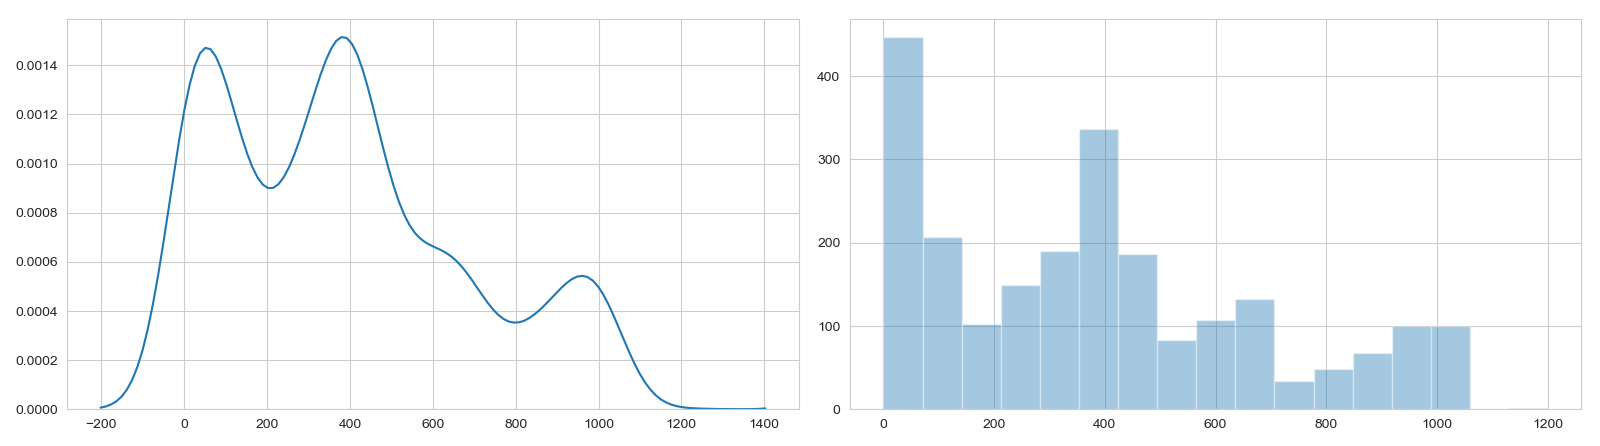
\includegraphics[width=\textwidth]{./Figures/edwin-Fake_certificate_survival_distribution3_new.png}
    \caption{仿冒应用应用证书活跃时间分布}
    \label{fig:Fake_certificate_survival_distribution}
\end{figure}

按~\secref{sec:behavior_method}所述方法计算证书活跃时间,~\autoref{fig:Fake_certificate_survival_distribution}展示了不同仿冒应用应用证书在应用市场里活跃时间的总体分布。
考虑到上节结果显示76\%应用证书仅关联一至两个仿冒样本,对活跃时间计算有较大干扰(仅发布一个样本的证书活跃天数为0天),图中数据去除了该部分数据。
左图为概率密度分布图,$x$轴表示活跃时长,$y$轴表示了与$x$轴上的值对应的概率密度。
右图为数量分布直方图,$x$轴表示活跃时长,$y$轴对应区间内证书数量。

经计算,~\autoref{fig:Fake_certificate_survival_distribution}左图中$x$轴值大于109对应的$y$轴曲线下方区域面积接近0.75,表示约75\%仿冒应用应用证书活跃时间大于109天,数据的50分位数与75分位数分别为366与579.5,表示50\%仿冒应用证书活跃时间超过一年,约25\%仿冒证书活跃时间超过580日。
前文提及的证书``\emph{61ed377e85d386a8dfee6b864bd85b0bfaa5af81}''也是活跃市场最长的应用证书。
本研究采用的仿冒样本上架时间范围为2015年5月29日至2018年9月15日之间,使用上述证书签署的样本最早于2015年11月12日在百度手机助手上架,最晚于2018年9月15日在百度手机助手上架。
2015年至2018年间,该证书一直处于活跃状态,29个渠道中,除Uptodown,天翼应用市场、Apkpure、GiONEE、中移动应用商店、Google Play应用商店6个应用市场中未有发现由该证书签署的样本外,其他23个应用来源均有发现与该证书关联的样本。
然而,三年期间发布1,374个样本是有违常理的,以一年365天计算,需在每1.25日开发、上架一个新应用样本,该开发速度与日常认知并不一致。
而且,该证书为Android Studio内置调试证书,因此作者认为证书对应的1,374个样本并非由同一个人或组织上传。
进一步推断,各市场除了接收应用开发者上传的应用外,还会自行搜集应用上架,但在搜集过程中并未制订严格安全规范,扩大了安全风险。

以上结果进一步表明国内应用市场防御机制存在较大缺陷,国内应用市场用户的利益并未能被有效保障。

\subsection{仿冒应用上架特征分析}

\noindent{\bf RQ6:仿冒应用的上架是否有特征?}

仿冒应用上架特征可分为不同角度观察:从宏观角度,仿冒应用上架数是否有一定趋势?从微观角度看,仿冒应用开发者上架应用时是否有偏好?
本节研究将RQ6细分为以下子问题:

{\bf RQ 6.1}:仿冒应用总体上架量是否呈现一定趋势?

{\bf RQ 6.2}:仿冒应用开发者是否会同时在多个市场上架应用?

{\bf RQ 6.3}:仿冒应用开发者偏向在新应用版本推出多久后发布仿冒应用?

\noindent{\bf RQ 6.1}:仿冒应用总体上架量是否呈现一定趋势?

\begin{figure*}[t]
    \centering
    \subfloat[每月仿冒样本数量\label{fig:sample_cnt_per_month}]{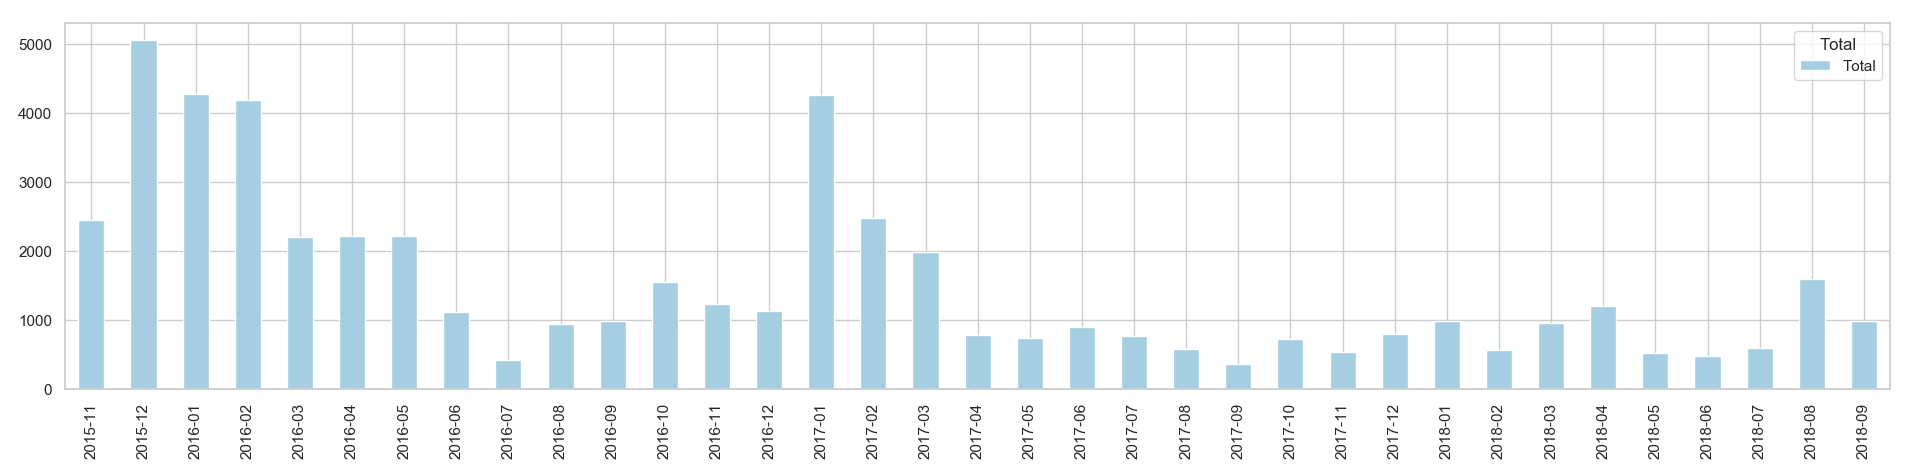
\includegraphics[width=\textwidth]{./Figures/edwin-Number_of_samples_collected_per_month.png}}\hfill

    \subfloat[每月活跃证书数量\label{fig:cert_cnt_per_month}]{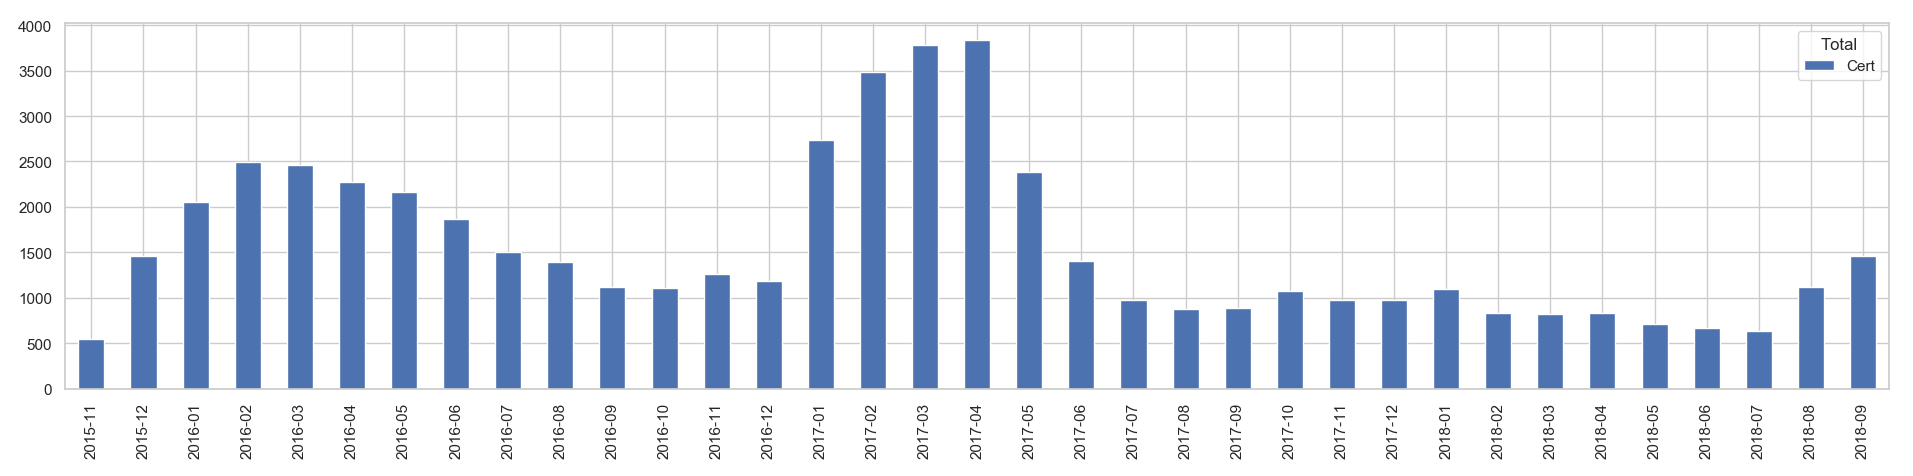
\includegraphics[width=\textwidth]{./Figures/edwin-Number_of_active_cert_per_month.png}}\hfill
    \caption{每月仿冒样本数量、应用证书数量(2015年11月至2018年9月)}
    \label{fig:fake_cnt_per_month}
\end{figure*}

图~\autoref{fig:sample_cnt_per_month}展现了自2015年11月起,仿冒应用开发者每个月在29个数据来源中上架的仿冒样本数量,$x$轴代表月份,$y$轴表示某月对应仿冒样本数量。
数据表明,2015年年末、2016年第一、第二季度与2017年第一季度间,有大量仿冒应用被上架到市场中,其他时段仿冒应用上架量较为稳定,约为每月1,000个,仿冒应用上架量有逐年递减的趋势。
图~\autoref{fig:cert_cnt_per_month}则为同时期在三个月内发布过仿冒样本的应用证书数量。
2016年与2017年第一、二季度为仿冒应用开发者最活跃的阶段,其后仿冒应用开发者数量骤减并趋向稳定,从2018年第三季度开始有复苏迹象。
结合两图,作者认为仿冒应用高峰已过,但其威胁依然存在,各大应用市场方仍需加强审查保障用户安全。

\noindent{\bf RQ 6.2}:仿冒应用开发者是否会同时在多个市场上架应用?

\begin{table}[htbp]
    \renewcommand{\arraystretch}{1}
    \footnotesize
    \centering
    \caption{仿冒应用证书多市场上架情况统计}
    \vspace{1mm}
    \begin{tabular}{l cccccccccc}
        \toprule
        {\bf 同时上架市场数量} & 1     & 2     & 3     & 4    & 5    & 6    & 7    & 8    & 9    & 大于等于10 \\
        \midrule
        {\bf 应用证书数量}     & 5063  & 2368  & 983   & 488  & 237  & 130  & 91   & 45   & 24   & 30         \\
        {\bf 占总量比例(\%)} & 53.53 & 25.03 & 10.39 & 5.16 & 2.51 & 1.37 & 0.96 & 0.48 & 0.25 & 0.32       \\
        \bottomrule
    \end{tabular}
    \label{table:multi_market_statistic}
\end{table}

作者对所有仿冒样本的上架情况与其应用证书关联,得到如\autoref{table:multi_market_statistic}所示的仿冒应用证书多市场上架情况。
逾半数仿冒证书(53.53\%)仅会发布在一个市场中,近半数仿冒应用证书对应的应用会发布在多个市场。
结果表明,仿冒应用开发者会在多个应用市场中上架仿冒应用,各应用市场之间并未采取策略应对此类行为。

\noindent{\bf RQ 6.2}:仿冒应用开发者偏向在新应用版本推出多久后发布仿冒应用?

\begin{figure}[h]
    \centering
    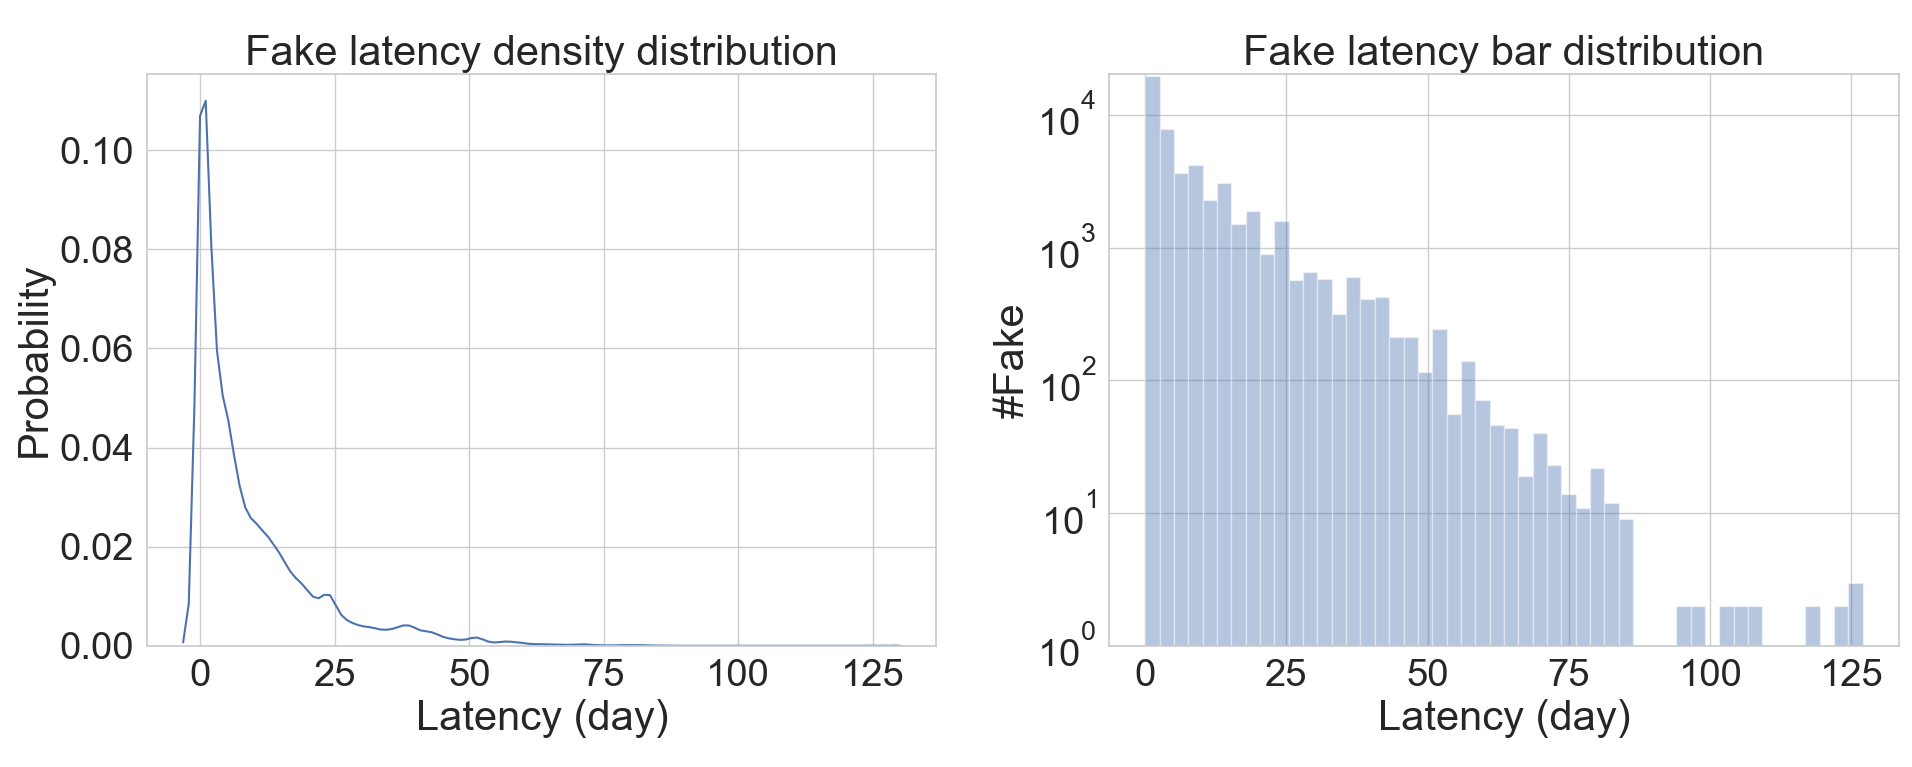
\includegraphics[width=\textwidth]{./Figures/edwin-Fake_latency_overall_distribution2.png}
    \caption{仿冒延迟总体分布}
    \label{fig:Fake_latency_overall_distribution}
\end{figure}

本研究按\secref{sec:behavior_method}中的方法计算了每版应用被仿冒的延迟时间和延迟的分布情况,结果显示如\autoref{fig:Fake_latency_overall_distribution}。
绝大多数(超过90\%)仿冒样本在官方新版推出后的20天内被发布,60\%仿冒样本在正版被推出的6天内发布,该结果表明仿冒开发者的行动十分迅速。
由于个人开发者的开发速度相对缓慢,作者推测制作仿冒应用已在移动黑灰产业中已规模化、组织化,以在新版应用推出后迅速推出对应的仿冒应用。
同时,根据\fullref{chp:discoveries_basic}结论,多数仿冒应用为重新开发的简单应用,而非重打包版本。
无需对原版应用进行破解、重打包也可加速仿冒应用开发流程,有利于仿冒应用开发者快速完成新版仿冒应用。

\subsection{研究结果有效性分析}

结构有效性已在上一节讨论过,不再赘述。

内部有效性威胁在于研究未能将仿冒应用证书与仿冒应用开发者精确匹配。
应用证书与开发者之间存在多对一关系,开发者创建证书时可输入名称等信息,但该信息不足以唯一定位开发者。
本章研究利用证书中的开发者名称信息匹配证书与开发者,此方式有效性有限(仿冒应用开发者可在创建不同证书时输入不同虚假信息),但有一定效果(如\emph{addone}与\emph{mobcent}两个开发者名称分别对应证书125个和195个,为仿冒应用开发者持有多个证书的论断提供数据支持)。
另外,上述多对一关系对RQ6.1研究的准确性也产生影响,每月实际活跃的仿冒应用开发者数量低于\autoref{fig:cert_cnt_per_month}所示的每月活跃证书数量。
然而,因数据显示仿冒应用证书活跃数下降趋势较为明显,~\autoref{fig:sample_cnt_per_month}也呈现仿冒样本骤减现象,可认为RQ6.1的研究结果依然有效。

外部有效性威胁源于两方面:其一,由于本章研究的目标应用为最受欢迎的50款Android应用对应的仿冒应用,未包含较小众的Android应用,未能探明针对小众Android应用的仿冒应用开发者具备何种行为特征;
其二,因开发者可任意发布Android应用程序,为降低收集、整理样本的成本,研究数据来源大部分源于国内应用市场,研究结果未必适用于整个互联网环境。
因此,尽管样本数据较丰富、来源多样,本章研究的结论普遍性仍未完善。
作者将在未来工作中对两方面入手进行更多研究,进一步提升研究普适性。
% \subsection{案例 1. 持有官方应用证书的可疑样本}

% 在人工浏览数据时,本研究发现了一个具有可疑应用名的样本---该样本声称自己是一个``破解版''的应用。
% % Furthermore, we checked (1) if strange word (e.g., ``cracked") appears in our official samples' names, (2) whether or not an official app is signed by an official certificate from another developer, and (3) if one official sample has a suspicious package name.
% 因此,本研究针对所有69,614个持有官方证书的样本进行了以下筛选:
% \begin{enumerate}
%     \item 使用``破解''、``免费''等关键字搜索所有带正版证书的样本,筛选出带有可疑应用名的样本;
%     \item 筛选所持应用证书与原开发者不一致的样本;
%     \item 筛选出包名和同款App的多数样本不一致的样本。
% \end{enumerate}

% % Eventually we acquired 17 suspicious official samples, listed in table~\ref{table:suspicious_samples} are samples in each of these three kinds.
% 最终,本文获得了17个由正版开发者应用证书签署的可疑样本,其中三个样本的信息如\autoref{table:suspicious_samples}中所示,分别代表上述三项筛选得到的结果。
% 第一个名为\texttt{爱奇艺}的样本虽然由一个官方应用证书签名,但该应用证书和其他爱奇艺样本的却不一致。
% 对比之后,本研究发现该证书来自360手机助手,但360和爱奇艺并没有合作关系,因此这是个可疑的样本;
% 而第二个样本(\texttt{360手机助手})的可疑之处在于样本包名。多数\texttt{360手机助手}的包名为\emph{com.qihoo.appstore},也有少部分官方包名为\emph{com.qihoo.secstore},前者为\texttt{360手机助手}在国内第三方应用市场发行的应用包名,后者为Google Play官方应用市场上上架的包名。然而,其中一个使用了其官方应用证书签署的样本的包名却是\emph{com.kuyou.sdbgj.baidu},十分奇怪;
% 第三个样本则是在应用名中包含了``破解''字样。然而,正常的正版应用根本不会有这样的命名方式,所以本研究也认为这是一个可疑样本。


% % \textsc{Virustotal} reports that only 2 of the 17 samples are benign, 2 are PUP and the other 13 samples are all malicious.
% \textsc{Virustotal} 的检查结果显示,17个可疑样本中,只有2个是良性应用,2个是PUP,余下13个样本都被判定具有恶意行为。
% 进行后续分析时,相关样本已被剔除出正版样本集合。

% \begin{table*}[htbp]
%     \renewcommand{\arraystretch}{1}
%     \small
%     \centering
%     % \setlength{\belowcaptionskip}{-10pt}
%     \caption{持有官方应用证书的可疑样本}
%     \begin{tabular}{l l c c c c c c}
%         \toprule
%         {\bf 样本应用名}               & {\bf 样本SHA1码}                         & {\bf 可疑之处} \\
%         \midrule
%         % 爱奇艺 & b86c55a509e8293b24138b166e9ff410f39e84b5 & 可疑证书(360手机助手) \\
%         爱奇艺                         & b86c55a509e8293b24138b166e9ff410f39e84b5 & 可疑证书       \\
%         % 360手机助手 & 2bb43c53b86d204d0040a8af6cb2a09cf9e93bb7 & 可疑包名(com.kuyou.sdbgj.baidu) \\
%         \rowcolor{gray!15} 360手机助手 & 2bb43c53b86d204d0040a8af6cb2a09cf9e93bb7 & 可疑包名       \\
%         % Youku XL 破解版 & b55b7ef189d649aeb03443c5d1ab57c9031d624e & 可疑应用名(``破解版") \\
%         Youku XL 破解版                & b55b7ef189d649aeb03443c5d1ab57c9031d624e & 可疑应用名     \\
%         \bottomrule
%     \end{tabular}
%     \label{table:suspicious_samples}
% \end{table*}

% % Despite the possibility that these certificates were somehow leaked to the underground industry, it is more likely that some attackers penetrated the protection scheme.
% 鉴于这17个样本都是持有官方应用证书签名的,有理由怀疑有应用厂家不慎泄露了自己的安全密钥库,从而导致了这些样本的出现。
% 然而,如果真的是因为厂家泄露密钥库,一来很有可能会导致恶意开发者使用官方应用证书大量生产恶意应用,二来对应厂家也会出于安全考虑马上更换新的包名和应用证书。
% 本研究的数据并不支持以上猜想带来的两点结果,所以本文不认为这是由于应用证书泄露导致了这些可疑样本的产生。

% 除去这个可能性,本文认为更有可能的原因是某些仿冒应用开发者掌握了穿透/绕过Android系统签名机制的技术,从而产生了这些样本。

% % As far back as December 2017, Google had confirmed and revealed a backdoor on V1 signature scheme (CVE-2017-13156)~\cite{android_security_bulletin}, by which hackers can inject any content into an apk at will without modifying its certificate information.
% 时间回溯到2017年12月,Google确认并公布了V1版本应用签名机制的一个后门(CVE-2017-13156)~\cite{android_security_bulletin}。
% 通过这个后门,黑客可以在不修改APK包应用证书信息的情况下,向APK包里注入任意内容。
% % An alternative solution, V2 signature scheme, has been launched at least one year before that.
% 而早在这个漏洞被公布的至少一年之前,Google就已经发布了作为V1版签名机制的替代解决方案,也就是V2版应用签名机制。
% % In order to confirm if these apps are using the risky V1 scheme, we used a tool, apksigner, provided by Google to verify which signature schemes these samples are using.
% 这看起来十分有可能是导致这些可以样本产生的原因,某些恶意开发者利用了V1版本签名机制的漏洞,修改了APK包的基本信息。
% 为了确认这些样本是否采用了具有风险的V1版应用签名机制,本文使用了apksigner来检测这些样本使用的签名机制版本。
% apksigner是Google官方提供的一个命令行工具,它被集成在Android SDK中,既是APK包编译打包过程中为APK包进行数字签名的工具,也可以用来验证APK包使用的签名机制版本,又或者是验证APK的签名是否有效。

% % It ends up that all 17 samples are using V1 signature scheme.
% apksigner的结果显示,所有17个样本都只使用了V1版本的应用签名机制。
% % With actually knowing that V1 is no longer safe, developers still refuse to embrace the safer scheme, which is really disappointing.
% 在了解到V1版本签名机制已经不再安全的情况下,仍有部分开发者由于各种原因没有接受更新也更安全的签名方案,这个结果令人失望。

\section{相关工作对比分析}

与本节工作相关的研究分为两类,一类的研究方法与本章类似,另一类的研究目的与本章类似。

Zhang等人针对Android应用中的第三方库进行实证研究~\cite{zhang2020empirical},其中采用了与本文类似的研究方法,探究应用作者与潜在恶意第三方库(Potentially Malicious Libraries,PMLs)的关联。
该文献提取应用中的证书信息,与应用中的PML进行配对,寻找与PML存在一对一关系的应用证书,并推断某些流行的PML可能由同一开发者制作。
在探究PML与应用证书的关联时,Zhang等人也发现了其应用样本包含开发者名为空或为Android Debug的证书。
由于该类证书无法提供更多开发者信息,Zhang等人将携带该类证书的应用从研究中排除。
与之相比,本研究重点为通过分析仿冒应用作者的行为揭示应用市场现存的监管漏洞,此类证书的出现表示应用市场在应用证书审核流程仍有缺陷,与研究方向相符,因此本章研究并未筛去此类证书及相关样本。

与本文研究目的类似的工作有Zhang等人针对Android恶意应用的实证研究~\cite{Zhou2012DissectingAM}。
该文献收集了源于49个家族的1,260个Android恶意应用,结合数据统计与样例分析,总结出与恶意应用相关的领域知识,如恶意应用常通过重打包、更新攻击和路过式下载(Drive-by Download)三种方式进行传播。
更新攻击指恶意应用开发者为了躲避应用市场的监管审查,有意在应用市场上上架不包含恶意代码的应用,然后在用户安装应用之后,提示用户升级,进而绕开应用市场,将带有恶意代码的新版本安装到用户设备上的行为。
路过式下载则指用户已安装的恶意软件,在用户不知晓的情况下,静默下载和安装更多恶意软件的行为。
通过揭示恶意应用的传播方式、恶意行为等信息,该研究揭示了改良已有恶意应用检测方法的重要性与优化方向。
类似地,本文通过对大量仿冒应用数据分析挖掘,点明现阶段应用市场的监管机制、策略缺陷,也可为应用市场方提供风险管控参考方向。


\section{本章小结与实用建议}
本章分别从仿冒应用与开发者的对应关系、仿冒应用证书活跃时间与仿冒应用上架特征三个不同视角对数据进行分析,结果可总结如下:
从仿冒应用与开发者的对应关系看,一个仿冒应用作者可持有多个应用证书,每个证书仅用于上架少量应用,这可被视作绕开应用市场监管机制采取的策略;
同时,部分仿冒应用作者采用Android调试证书在应用市场上架仿冒应用,但应用市场并未拦截此类行为。
从仿冒应用证书活跃时间看,去除仅上架了少量应用的证书后,数据显示仿冒应用证书能在较长时间保持活跃。
该结果表示,国内应用市场未能有效发现、处理上架了仿冒应用的开发者,监管机制存在较大缺陷。
从仿冒应用上架特征角度看,数据表示仿冒应用行业在2016、2017年发展迅速,有大量仿冒应用上架、大量证书活跃。
行业热度在2018年有回落趋势,但在2018年第三季度起有复苏迹象;
数据显示近半数仿冒应用于多个应用市场中上架,表示各应用市场间未有交流机制以共同抵御仿冒应用;
仿冒应用可在正版应用新版发布后迅速推出,表示仿冒应用产业链已较为成熟。

针对本章实证研究结果,对应用市场方有三点实用建议如下:
1)应用市场在审核开发者资质时,应加强对应用证书的检验,阻止开发者利用调试证书上传应用,并要求开发者上传具备完善、真实开发者信息的证书;
2)为对抗仿冒应用威胁,应用市场应完善监管机制,加快对仿冒应用开发者的处理,禁止曾上传过仿冒应用的开发者账号利用同一证书再上传应用;
3)恶意开发者/可疑开发者信息互通平台缺失,导致仿冒应用开发者可在多个应用市场上架仿冒应用,各应用市场应尽快合作建立类似平台,联合监管国内Android生态环境。
% \vspace{5mm}
% \noindent\fbox{
%     \parbox{0.95\linewidth}{
%         % \textbf{Remark 1}: Most certificates link with only a number of fake apps, which is highly possible to be a fake developers' evasive strategy.
%         \textbf{本节小结}: 绝大部分应用证书只与少数仿冒样本有所关联。这很可能是仿冒开发者规避市场监管机制采用的策略。
%         % Moreover, we observe that fake apps do tend to use official app names or names alike.
%         同时,本文也观测到仿冒应用倾向于于官方App相同或者是十分相似的应用名。
%         % Nonetheless, fake apps and official apps are not resemble in terms of package names or apk sizes, disclosing that repackaged apps are not mainstream in fake apps.
%         但是,仿冒样本和官方App在包名和APK包大小方面都不相似,这表明重打包应用在仿冒应用中并不普遍存在。
%         最后,如果良性应用的开发者不遵从最新的安全标准发布应用,可能会导致十分严重的安全问题。
%     }
% }